\documentclass{beamer}
%% Possible paper sizes: a0, a0b, a1, a2, a3, a4.
%% Font sizes can be changed using the scale option.
\usepackage[size=a1,orientation=portrait,scale=2]{beamerposter}
\usetheme{MAKposter}
\usecolortheme{RusLTC}
\usepackage{url}
\usepackage[utf8]{inputenc}
\usepackage[T1,T2A]{fontenc}
\usepackage[english,russian]{babel}
\usepackage{tempora} % this is the only package that does not produce errors related to font size with T2A 
\usepackage[scaled=0.92]{inconsolata}
\usepackage[libertine]{newtxmath}

\usepackage{mwe} %minimal working example

% \setbeamertemplate{itemize/enumerate body}{\tiny}
\setbeamerfont{itemize body}{family=\rmfamily, size={\fontsize{5}{7}}}
\setbeamertemplate{enumerate item}{\tiny\insertenumlabel.}

\usepackage{hyperref}
\hypersetup{
	colorlinks=true,       % false: boxed links; true: colored links
	urlcolor=cyan           % color of external links
}

\author[Research Group in Computational Linguisstics, UK]{RusLTC at RANLP-2019}
\title{Russian Learner Translator Corpus 2.0 \\ https://rus-ltc.org}
%\institute{}
% \subtitle{bigger and better}
% Optional foot image
\footimage{
\includegraphics[width=10cm]{images/ranlp2019.jpg}} %width=6cm

\begin{document}
\begin{frame}[fragile]
\begin{block}{RusLTC} %cyrilic letters in blocktitles produce errors if the size of the poster is changed inc. thru scaling
\large
\textbf{Parallel English<>Russian sentence-aligned corpus of multiple student translations.}
\end{block}
\vspace{-.5em}
\begin{columns}[T]
%%%% First Column
\begin{column}{.55\textwidth}

\begin{block}{Corpus size and metadata}
\begin{columns}
	\begin{column}{.5\linewidth}
		\begin{itemize}
			\item Basic statistics:
			\begin{itemize}
				\item \alert{2.3 mln words}, 4.8K texts;
				\item 402 English source texts, $\approx 8$ Russian translations for each;
				\item RU targets: $\approx$ 380 words.
			\end{itemize}
			\item Metadata:
			\begin{itemize}
				\item \alert{Translation grade}; %(32\%, 1.5K texts)
				\item Draft / final translation (editing effort);
				\item Routine / \alert{Exam / Contest}; % (36\%)
				\item At class / at home.
			\end{itemize}

		\end{itemize}
		
	\end{column}
	
	\begin{column}{.5\linewidth}
		\begin{itemize}
			\item Source text genres:
			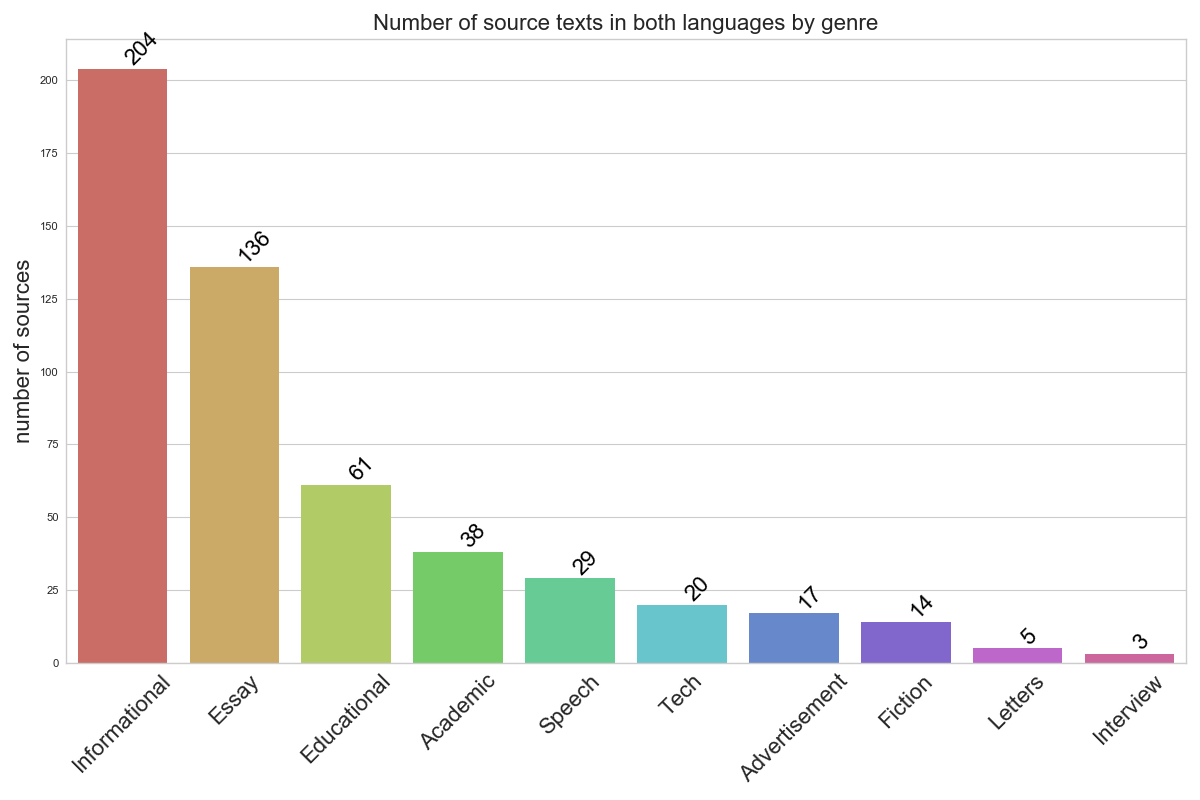
\includegraphics[width=\linewidth,keepaspectratio]{images/genres-desc_hls_oct2018.png}
			\item Translators:
			\begin{itemize}
				\item Gender-annotated;
				\item 60\% by advanced Translation Studies students;
				\item 14 Russian universities.
			\end{itemize}
		\end{itemize}
	\end{column}
		
\end{columns}
\end{block}

\begin{block}{New search interface: \\ElasticSearch + Tsakonian Corpus Platform}

\begin{columns}
\begin{column}{0.4\textwidth}
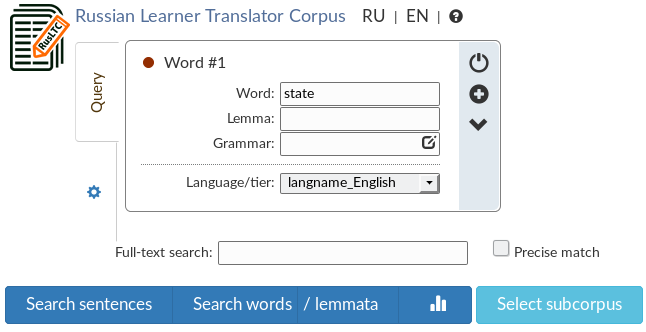
\includegraphics[width=\linewidth,keepaspectratio]{images/rltc_example.png} 
\end{column}
\begin{column}{0.55\textwidth}
\begin{itemize}
\scriptsize
    \item\textbf{ \textit{`Elected last October, he comes to office at a time when Latin America is in a state of upheaval.'}}
    \begin{enumerate}
    \tiny
   \item \textit{`После выборов в октябре прошлого года он пришел к власти, в это время в Латинской Америке были беспорядки.'}
    \item\textit{ `Он был избран в октябре и сразу столкнулся с проблемой экономического спада в Латинской Америке.'}
    \end{enumerate}
\end{itemize}
\end{column}
\end{columns}
\bigskip
	\begin{itemize}
	\small
		\item Search by lemmas and PoS:
		\begin{itemize}
		\footnotesize
			\item \textit{Do students find concise ways of rendering N+to+V\textsubscript{inf}?}
			\item \textit{Do students overuse existential verbs?}
		\end{itemize}
		\item Filtering by metadata (arbitrary subcorpora):
		\begin{itemize}
		\footnotesize
			\item \textit{Do advanced students use pronouns less?}
			\item \textit{Do they translate `in fact' and `people' in more different ways?}
		\end{itemize}
	\end{itemize}
	%\textbf{Try it out!}


\end{block}
\end{column}

%%%% This is the SECOND column
\begin{column}{.4\textwidth}

\begin{block}{Formats and availability}
\begin{itemize}
				\item Plain text documents;
				\item \alert{TMX} (XML-based bitext format);
				\item stand-off error annotation files;
				\item fully public, downloadable, CC-BY-SA.
				%\item names: EN\_1\_36.head.txt -- RU\_1\_36\_1.ann
\end{itemize}
\end{block}

\begin{block}{Error-annotated translations}
			\begin{itemize}
				\item $ > 750$ texts, 300K words, 16K error labels
				\item 30 error types, 3 weights, 10 tech attributes
				\item Annotated in \textbf{brat}:
			\end{itemize}

\begin{figure}
    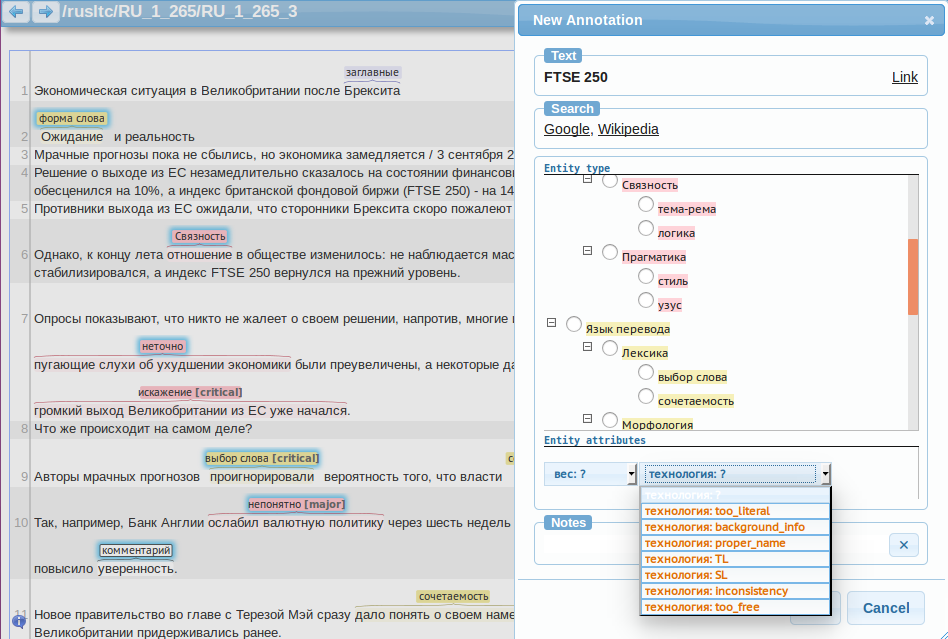
\includegraphics[scale=0.5,keepaspectratio]{images/brat.png}
\end{figure}

\textbf{Translation error types:}
\begin{figure}
    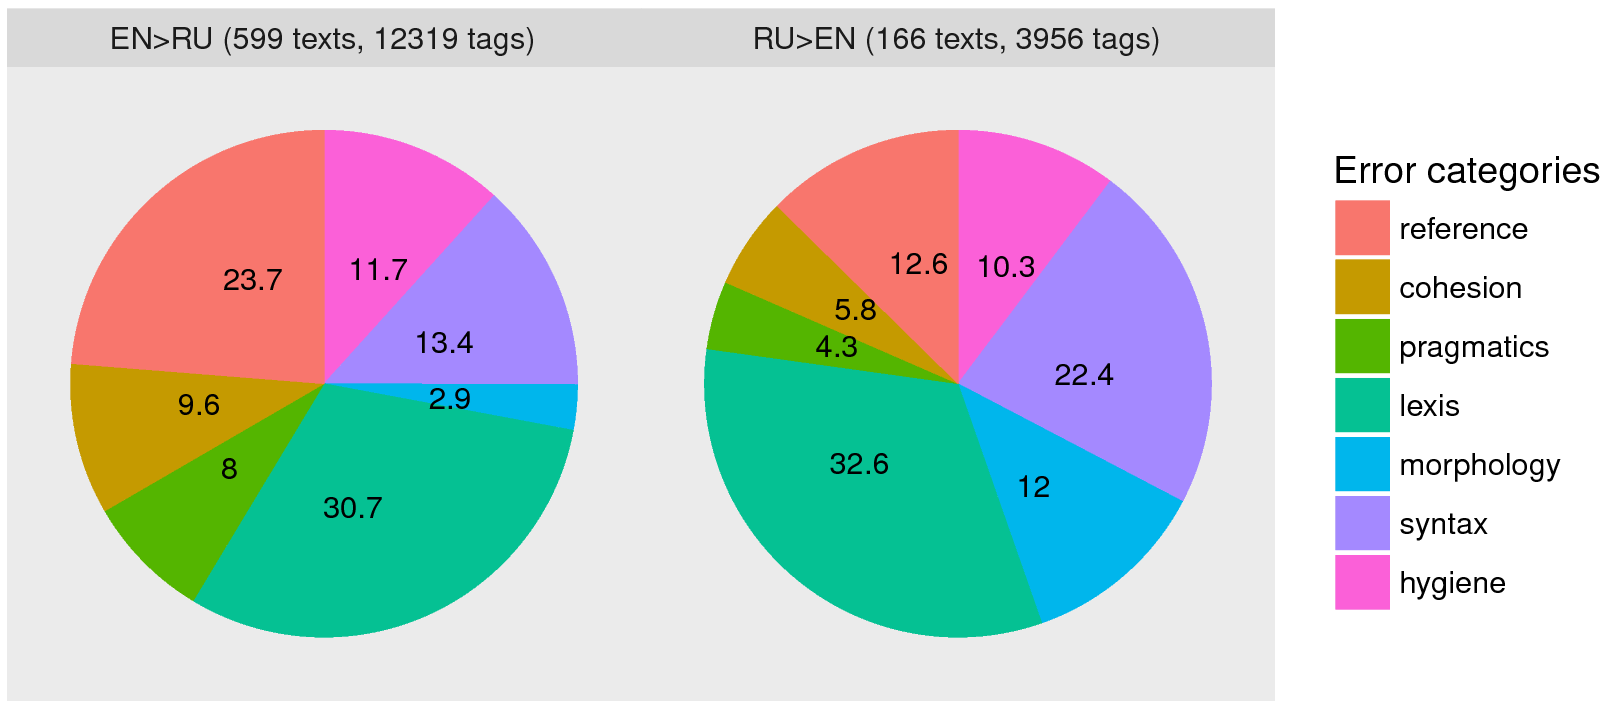
\includegraphics[width=0.7\linewidth,keepaspectratio]{images/error.png}
\end{figure}
\end{block}

% ????
%\begin{block}{Comparable prof and ref corpora}
%		\begin{itemize}
%			\item 50\% InoSMI parallel corpus (450K wds)
%			\item RNC newspaper filtered for local, OOD and short texts (3.5M wds)
%		\end{itemize}
%\end{block}
\end{column}
\end{columns}

  \begin{beamercolorbox}[wd=\paperwidth]{lower separation line head}
  	\rule{0pt}{0.2em}
  \end{beamercolorbox}
%\vspace{-.3em}
\centering
\Large{\textbf{\textcolor{Zen}{Some published research applications}}}
%\vspace{-.4em}

\setbeamercolor{block title}{fg=white,bg=HazySummerEve!60}
\setbeamercolor{block body}{fg=black, bg=Again!60}
\small{\begin{columns}
	\vspace{4em}	
	\begin{column}{.32\linewidth}
		\begin{block}{Testing distinctions}
				\alert{Learner vs. professional translations}
	\begin{columns}
		\hspace{.5em}
		\begin{column}{.5\linewidth}
		
				\begin{itemize}
					\item Sentence length, splitting.
					\item Types to tokens ratio (TTR).
					\item Frequent words distribution.
				
				\end{itemize}
		\end{column}
		\begin{column}{.5\linewidth}
				\begin{itemize}
				    \item Lexical density.
					\item Morphological forms distribution.
					\item Connectives and epistemic markers. %(regex annotation, pre-defined lists)
				\end{itemize}
		\end{column}
	\end{columns}
		\end{block}
	\end{column}

\begin{column}{.33\linewidth}
	\begin{block}{Translation types features}
		\begin{itemize}
			\item \alert{learner}: 200 texts, 206K words
			\item \alert{professional}: 200 texts, 326K words
			\item \alert{non-translations}: 1.5K texts, 3M words
		\end{itemize}
		\begin{columns}
		\begin{column}{0.5\textwidth}
		  \centering
		  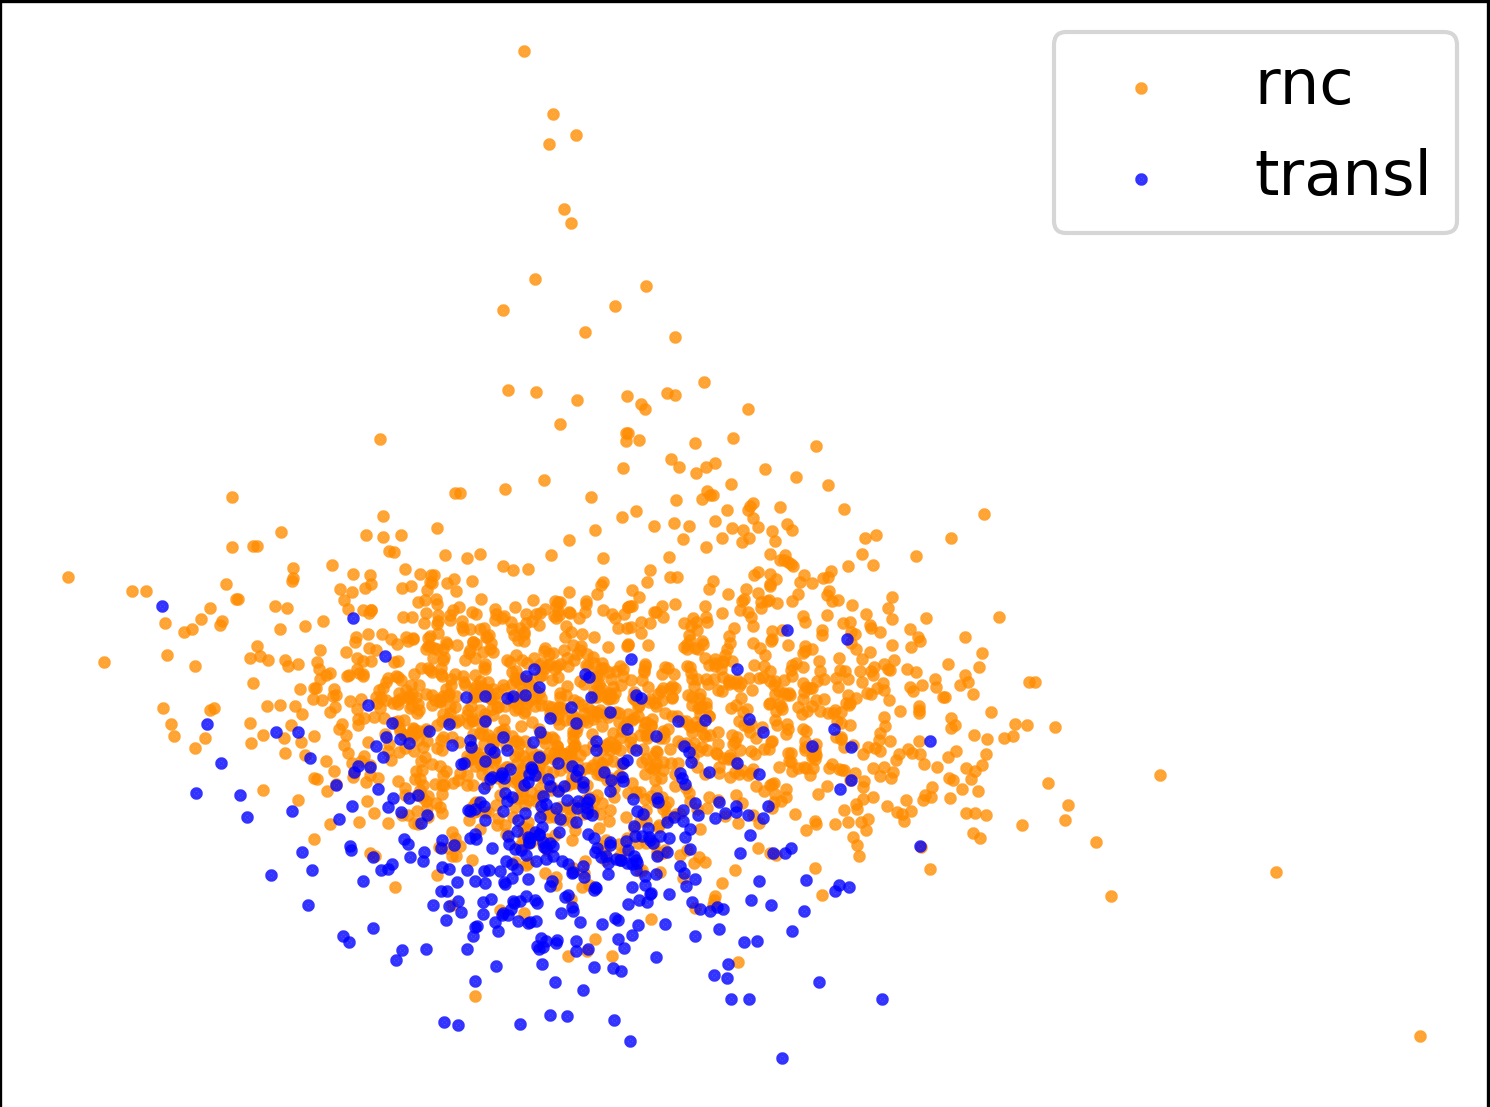
\includegraphics[width=0.5\textwidth,keepaspectratio]{images/2class_pca.png}
		\end{column}
		\begin{column}{0.5\textwidth}
		    \centering
		    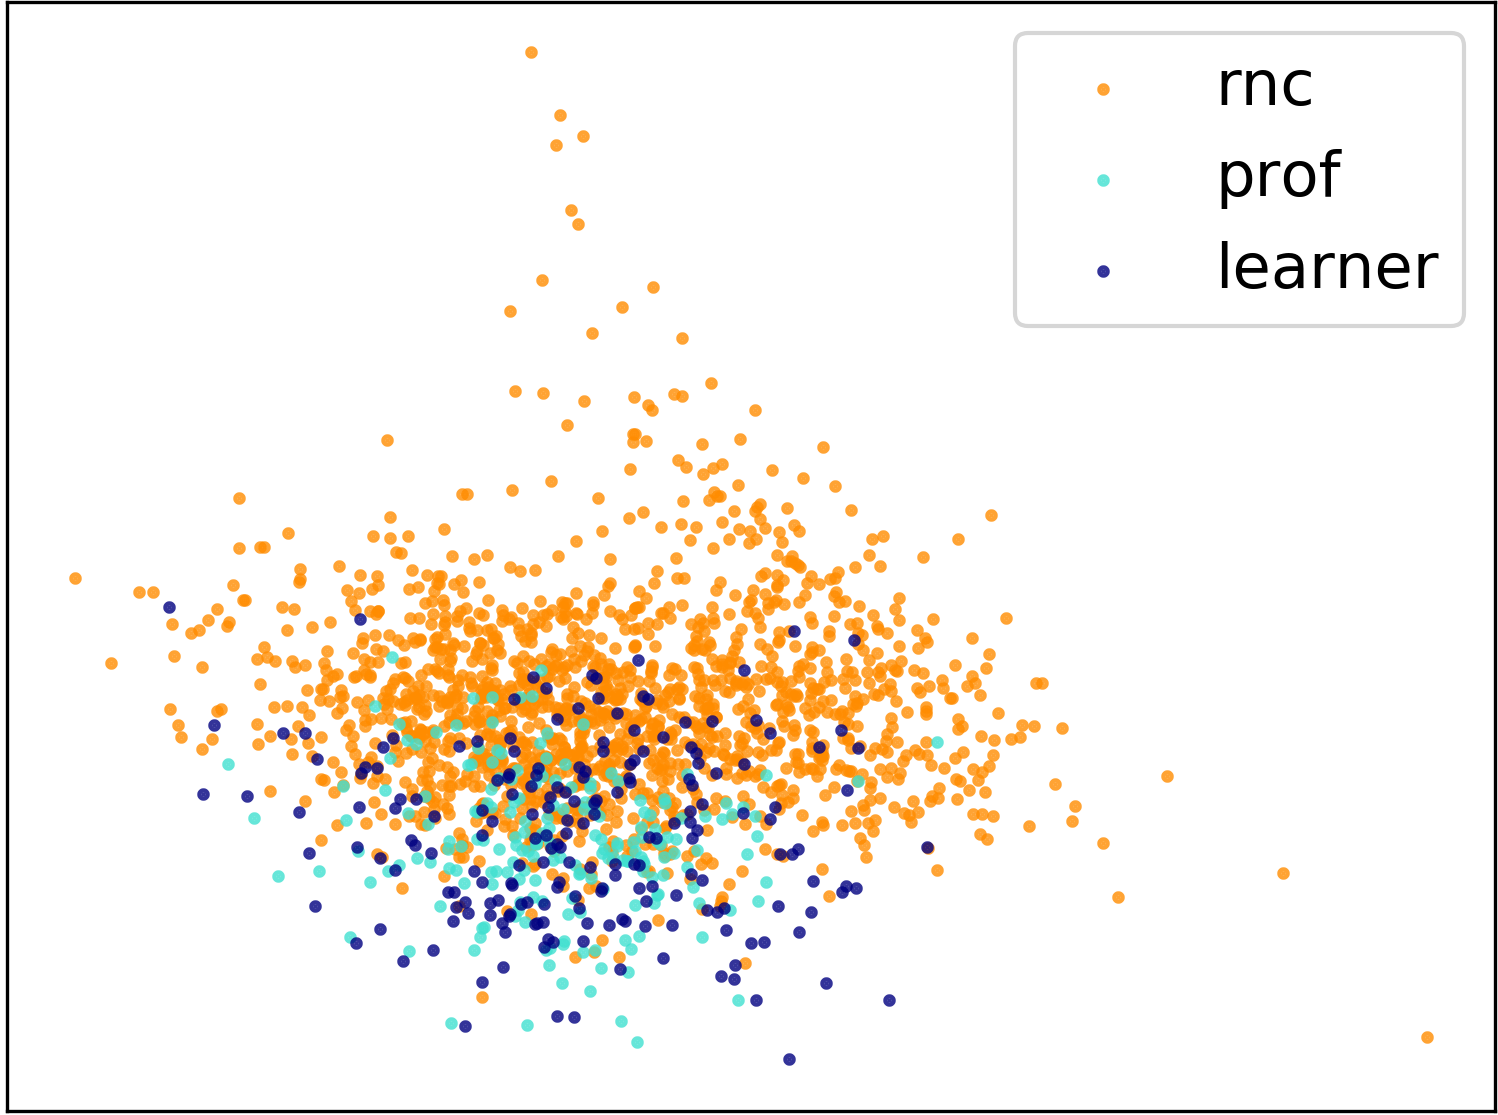
\includegraphics[width=0.5\textwidth,keepaspectratio]{images/3class_pca.png}
		\end{column}
		\end{columns}
			%	\item F1 score 86.6%, outperforms SOTA.
More explicit pronoun subjects, more verb chains, more analytic passives, etc.
\vskip-.3em
	\end{block}
\end{column}

\begin{column}{.30\linewidth}
	\begin{block}{Textbooks vs. real errors}
	\textbf{Data}: (1) annotated multiple translations to \alert{difficult sentences} from English mass-media, and (2) \alert{38 textbooks} for translation students (published in 1963-2016)
		\vskip.5em
		\begin{itemize}
			\item Of the top 20 most active error-triggers only 3 are discussed in the textbooks! 
		\end{itemize}
	\end{block}
\end{column}

\end{columns}}

\vfill

\setbeamercolor{block body}{bg=AlwaysBeBabyToMe!50,fg=black}
\setbeamercolor{block title}{fg=HazySummerEve,bg=WinterSkin}

\begin{block}{Plans and Outlook}
\begin{itemize}
\item \alert{Evaluate translation (alignment) accuracy}: similarity between source sentences and their correct and erroneous translations.
%(\textit{compositional distributional semantics}).
\item \alert{Lexical} level: collocations.
\item More \alert{syntactic} suspects: word order and constructions.
\item Comparison to \alert{machine translation}: 
\begin{enumerate}
    \item  non-human semantic and coherence errors,
    \item  professionalism is about fluency.
\end{enumerate}

\end{itemize}
\end{block}

\end{frame}
\end{document}